%%%%%%%%%%%%%%%%%%%%%%%%%%%%%%%%%%%%%%%%%
% Vertical Line Title Page
% LaTeX Template
% Version 2.0 (22/7/17)
%
% This template was downloaded from:
% http://www.LaTeXTemplates.com
%
% Original author:
% Peter Wilson (herries.press@earthlink.net) with modifications by:
% Vel (vel@latextemplates.com)
%
% License:
% CC BY-NC-SA 3.0 (http://creativecommons.org/licenses/by-nc-sa/3.0/)


\documentclass[a4paper, 11pt]{book} % A4 paper size and default 11pt font size
\usepackage[utf8]{inputenc} % Required for inputting international characters
\usepackage[T1]{fontenc} % Output font encoding for international characters
\usepackage{stix} % Use the STIX fonts
\usepackage{graphicx}
\usepackage{mathtools}
\usepackage{setspace}
\usepackage{hyperref}

%code to adjust margins
\addtolength{\oddsidemargin}{-.875in}
	\addtolength{\evensidemargin}{-.875in}
	\addtolength{\textwidth}{1.75in}

	\addtolength{\topmargin}{-.875in}
	\addtolength{\textheight}{1.75in}

\makeatletter

\begin{document}

%----------------------------------------------------------------------------------------
%	TITLE PAGE
%----------------------------------------------------------------------------------------

\begin{titlepage} % Suppresses displaying the page number on the title page and the subsequent page counts as page 1
	
	\raggedleft % Right align the title page
	
	\rule{1pt}{\textheight} % Vertical line
	\hspace{0.05\textwidth} % Whitespace between the vertical line and title page text
	\parbox[b]{0.75\textwidth}
	{ % Paragraph box for holding the title page text, adjust the width to move the title page left or right on the page
		
		{\Huge\bfseries MATH 310  \\[0.5\baselineskip] Probability \& Statistics}\\[2\baselineskip] % Title
		{\large\textit{Project Observations}}\\[4\baselineskip] % Subtitle or further description
		{\Large\textsc{muhammad munawwar anwar (ma04289) \\ khubaib naeem kasbati (kk04333) }}\\[2\baselineskip] % Author name, lower case for consistent small caps 
		 % Author name, lower case for consistent small caps
		 {\Large\textsc{Github Repository : }} \href{https://github.com/khubaibkay1/ProbabilityRandomWalks}{Probability Random Walks}\\[2\baselineskip]
        {\large June 19, 2020}\\[2cm] % Date, change the \today to a set date if you want to be precise
		\vspace{0.5\textheight} % Whitespace between the title block and the publisher

		{\noindent Habib University}\\[\baselineskip] % Publisher and logo
		
	}
	
    
\end{titlepage}
%----------------------------------------------------------------------------------------
\tableofcontents


\addcontentsline{toc}{chapter}{Figures}
\listoffigures


\newpage

\addcontentsline{toc}{chapter}{Tasks}
\section*{Tasks}


\addcontentsline{toc}{subsection}{Task 1}
\subsection*{Task 1}

In task 1, we ran the simulation 100,000 times, where each simulation consisted of 50 steps and the probability for the walk to move left, right or stay equally likely and the starting position was the point zero,  the expected value of the distance travelled was \(0.00992\) .The resulting distrubution can be found in Figure \ref{fig:task1}.
Furethermore, the distrubution was symmetric about the mean value. However, if the chosen starting point is not zero or the probability to move left, right or stay is unequal then the mean of the distrubution shifts or it becomes left or right skewed.
\\
We know that this simulation is valid since a gaussian distrubution is formed due to the Law of Large numbers and the expected movement at each turn is 0. \(E(X)= \frac{1}{3} \times-1 + \frac{1}{3} \times 0 + \frac{1}{3} \times 1 =0\) and hence \(E(50X)= 50 E(X) =0\), Due to linearity of expectation and because each event is independent. This matches the result we achieved empirically.
\addcontentsline{toc}{subsection}{Task 2}
\subsection*{Task 2}

In task 2 we the ran the simulation 10000 times, where in each simulation the starting distance x between two people was 100 and the probability for the both person to move left, right or stay was equally likely and same, the expected value of time required for both people to meet was \(8468.63\) . The distribution can be seen in Figure \ref{fig:task2}.
The distrubution is left skewed. (If we change the probabilities it will change skewness and changing the initial distance shifts the center of the graph)  The starting distance x between the two people appears to have a  linear relation with number of time required to meet. \\
Our model is based on the assumption that there exists some outliers. And excluding them would not effect the expected value by much. We have added a timeout and if the simulation fails in that time then we ignore that simulation, this can lead to a correct average when the timeout is set accordingly but for large distances it can distort the real expected value by causing the simulations with near expected time to timeout.


\addcontentsline{toc}{subsection}{Task 3}
\subsection*{Task 3}

Suppose that a walker is at the position $P = (P_1,P_2)$ inside the test region at $(k-1)^{th}$ step, but
the next step would be to a position $ Q = (Q_1,Q_2) $ that is either on the boundary or beyond the 
boundary. We divide the contemplated step from P to Q into two steps  : (1) an
actual step (the $k^{th}$) to the boundary point $P^{\prime}$,where the segment $\vec{PQ} $ intersects the boundary,  and then (2)
a step $(k+1)^{st}$ of one unit to a point $Q^{\prime}$ inside the circle. Specifically, let $P^{\prime}$ be the
point where the walker hits or would cross the boundary and $\alpha$ the angle of incidence of the walker's path
with the tangent line to the circle at  $P^{\prime}$. The walker takes a step (kth step) to $P^{\prime}$ and then takes a step((k+1)st) back into the 
circle on a path which forms an angle $\alpha$ with the tangent line at $P^{\prime}$. This Reflection method can be seen in Figure \ref{fig:reflectionrule}.
The distribution of these points can be seen in Figure  \ref{fig:task4}
\\ The parameters used to create this distribution were \(0,0.5,1\) for r with equal probability each, and \(0,\frac{\pi}{2}, \pi\) with equal probability each. (Our code allows the users to change the parameters to their liking)





\addcontentsline{toc}{subsection}{Task 4}
\subsection*{Task 4}

Similar to task 1 when we the ran the simulation 10000 times, where each simulation consisted of 50 steps and the step was modeled as a uniform random variable between 0 and 1 , the expected distance in a particular step is 0.5 hence in 50 steps is 25. This matches with our empirical result of \(\approx 25.03 \)
Furthermore, the distrubution was symmetric about the mean value. However, if the chosen starting point is not zero or the probability to move left, right or stay is unequal then the mean of the distrubution shifts or it becomes left or right skewed. Shifting the start of the simulation by x units leads to the distribution being shifted by x units. The distribution can be seen in Figure \ref{fig:task4}.


\addcontentsline{toc}{subsection}{Task 5 \& 6}
\subsection*{Task 5 \& 6}
We have created a random walk model and ran a simulation 100,000 times with 10,000 steps each. With step size being a uniform random variable between 0 and 1, and angle as a uniform random variable between 0 and \(2 \pi\). The results were that the distrubution was very well spread around the center, with the x and y values having a gaussian distrubution. The most common points were near the center of the circle. This checks out since the expected movement in x,y direction is 0 per step. Hence throughout the origin, on average it should be near the origin.  The model has been carried forward from Task 3.
\[\int^{2\pi}_{0} \int^{1}_{0} r \cos (\theta) = 0\]
\[\int^{2\pi}_{0} \int^{1}_{0} r \sin (\theta) = 0\]
% \addcontentsline{toc}{subsection}{Task 6}
% \subsection*{Task 6}


\addcontentsline{toc}{subsection}{Task 7}
\subsection*{Task 7}
We have created a random walk model and ran a simulation 100,000 times with 10,000 steps each. With step size being a discrete random variable which takes the values $\{0,0.5,1\}$, with equal probability each (Our code however allows the users to change the parameters to their liking) and angle as a uniform random variable between 0 and \(2 \pi\). The results in task 7 were analagous to those in task 5 and 6. The distrubution was very well spread around the center, with the x and y values having a gaussian distrubution. Most of the points were near the center of the origin. The model has been carried forward from Task 3.
\addcontentsline{toc}{subsection}{Task 8}
\subsection*{Task 8}

In task 8, when we ran the simulations 14000 times the expect value of time that it takes for two nodes to meet was 111,504. 
The initial location of the model was chosen by using polar coordinates and modelling radius as uniform random variable
between 0 and 100 and the angle as a uniform random variable between 0 and $2\pi$. In order to determine the approriate number of simulations
required we will use 95\%  confidence interval and precision level at 2000. \\

\textbf{Level of Precision} : The maximum degree the true population mean can deviate from the sample mean estimation,subject to a given
confidence interval.

The confidence interval is calculated as follows :
$$ \text{CI} = (\bar{x} - z \times \frac{s}{\sqrt{n}},\bar{x} + z \times \frac{s}{\sqrt{n}} )$$ 
where $\bar{x}$ is the sample mean, $s$ is the standard deviation of the sample mean , $n$ is the sample and z is the statistic associated with a certain 
confidence interval. Since we have chosen a 95\% confidence interval, the z statistic equals to 1.96
approximately. \\

After some algebaric maniuplations , we can write the above equation as follows :
$$P(\frac{-\phi}{s\sqrt{n}}<\frac{\bar{x}-\mu}{s\sqrt{n}}<\frac{\phi}{s\sqrt{n}})$$
where $\bar{x}$ is the sample mean, $s$ is the standard deviation of the sample mean , $n$ is the sample size, $\mu$ population mean,and $\phi$
is the level of precision. \\

According to the Central Limit Theorem, the middle term in the above inequality is normally
distrubuted with mean zero and standard deviation one. Consequenlty, we can solve the lower and upper
bounds of the equation for the only unknown variable , n . \\

We know that s, the sample standard deviation , $ 117,551.58$ , $z = 1.96$ and $\phi = 2000$

$$ \sqrt{n} = \frac{1.96 \times 117,551.58}{2000} \text{ , so } n = 13,271 \text{ simulation} $$.

Since our sample distribution was not a normal distribution, the distribution of the sample variance was unknown. This means
that our answer we got for n, number of simulations is not the theoretical minimum. Although, a larger sample size means that the
distribution of sample variance approaches to the normal distribution.




 
\newpage
\section*{Figures}
\begin{figure}[h]
	\centering
	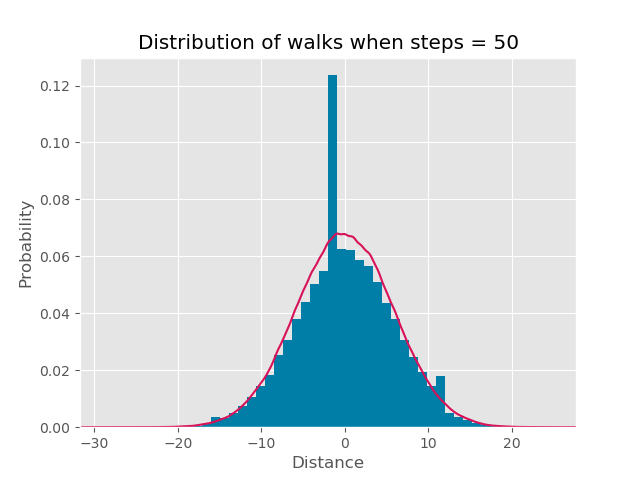
\includegraphics[width=0.7\textwidth]{Task 1.png}
	\caption{Task 1: One Dimensional Discrete Random Walk}
	\label{fig:task1}
\end{figure}

\begin{figure}[h]
	\centering
	\includegraphics[width=0.7\textwidth]{task 2.png}
	\caption{Tak 2: Distrubution of time required for two people who are intially 100 units away}
	\label{fig:task2}
\end{figure}
\begin{figure}[h]
	\centering
	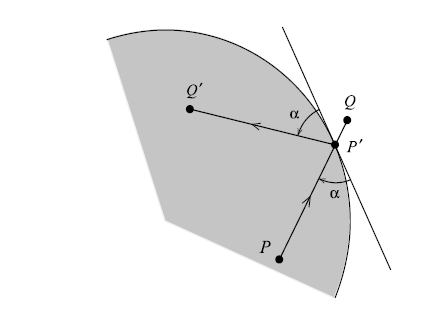
\includegraphics[width=0.8\textwidth]{ReflectionRule.png}
	\caption{Reflection from the Circumference}
	\label{fig:reflectionrule}
\end{figure}

\begin{figure}[h]
	\centering
	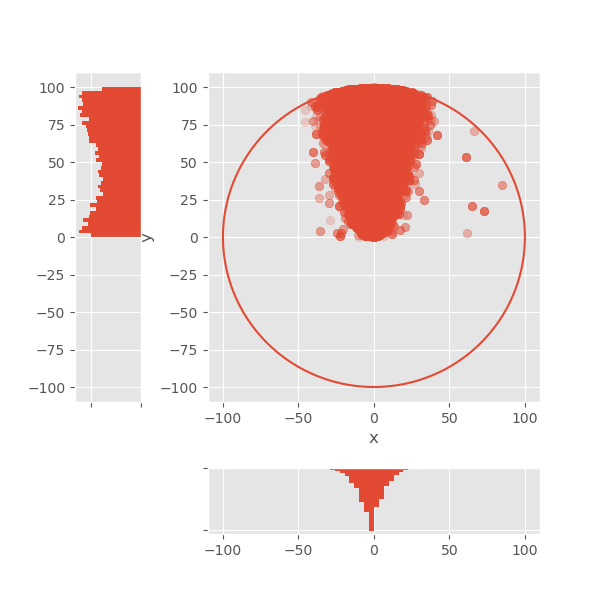
\includegraphics[width=0.8\textwidth]{Task3.png}
	\caption{Task 3: Two Dimensional Discrete Random Walk, with main graph showing distribution of the points after simulation, subgraph showing distribution of x (Below x axis) and a subgraph showing distribution of y (Left of y axis)}
	\label{fig:reflectionrule}
\end{figure}

\begin{figure}[h]
	\centering
	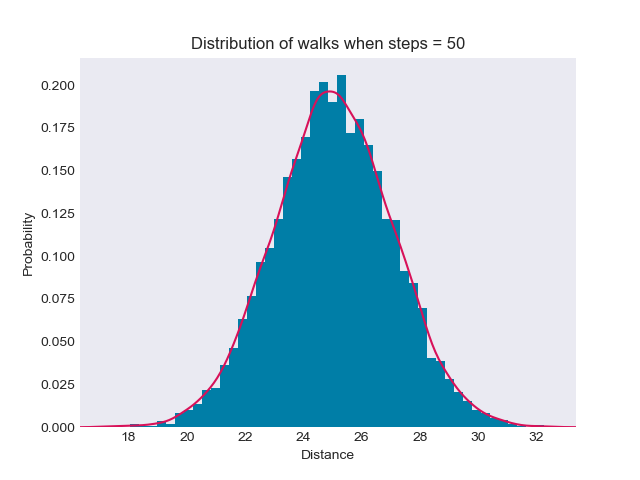
\includegraphics[width=0.8\textwidth]{task 4.png}
	\caption{Task 4: One Dimensional Discrete Random Walk , with main graph showing distribution of the points after simulation, subgraph showing distribution of x (Below x axis) and a subgraph showing distribution of y (Left of y axis)}
	\label{fig:task4}
\end{figure}

\begin{figure}[h]
	\centering
	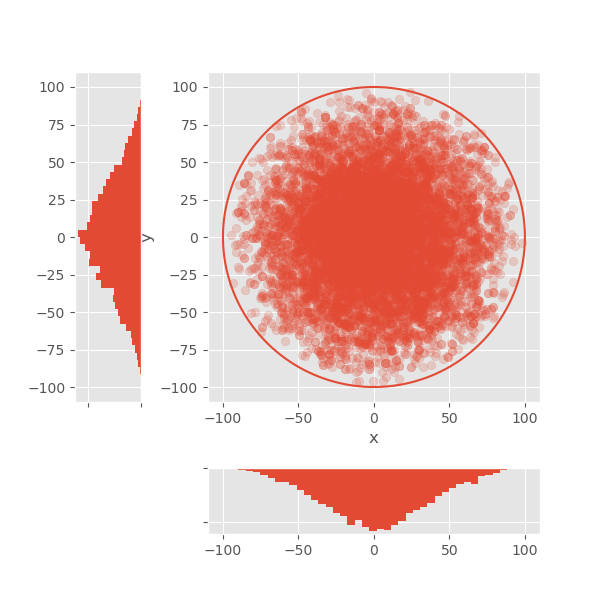
\includegraphics[width=0.8\textwidth]{Task5.png}
	\caption{Task 5 \& 6: Two Dimensional Continuous Random Walk, with main graph showing distribution of the points after simulation, subgraph showing distribution of x (Below x axis) and a subgraph showing distribution of y (Left of y axis)}
	\label{fig:task5}
\end{figure}

\begin{figure}[h]
	\centering
	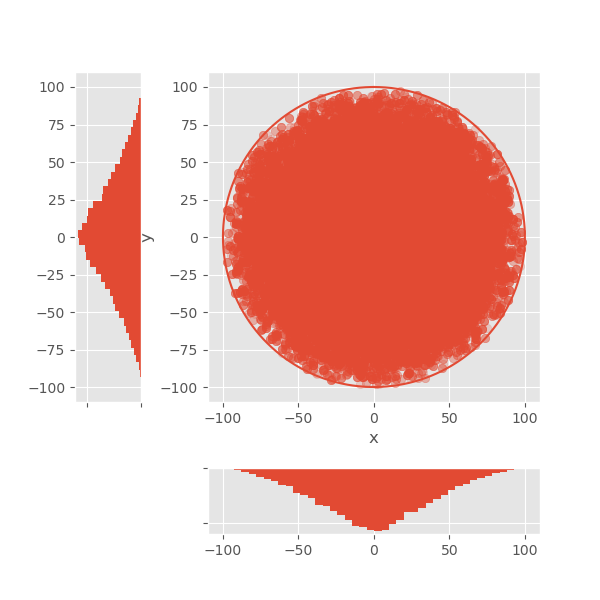
\includegraphics[width=0.8\textwidth]{Task7.png}
	\caption{Task 7: Two Dimensional Random Walk with Discrete Step Size and Continous Angle, with main graph showing distribution of the points after simulation, subgraph showing distribution of x (Below x axis) and a subgraph showing distribution of y (Left of y axis)}
	\label{fig:task7}
\end{figure}

\begin{figure}[h]
	\centering
	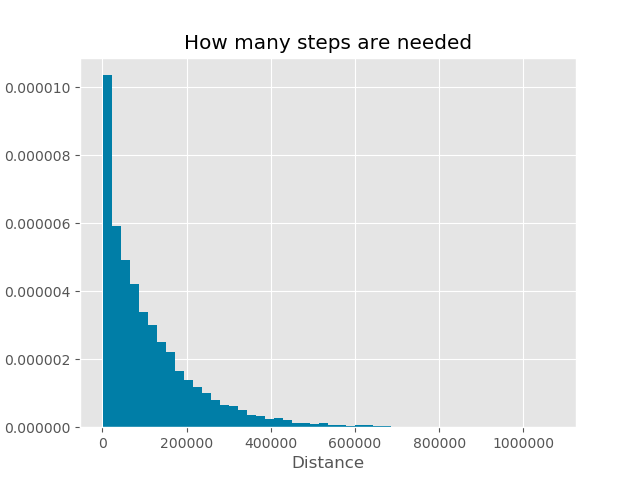
\includegraphics[width=0.8\textwidth]{Task8.png}
	\caption{Expected number of steps it would take for two nodes to meet.}
	\label{fig:task7}
\end{figure}


\newpage
\addcontentsline{toc}{chapter}{Bibliography}
\begin{thebibliography}{9}
    \bibitem{aa1} 
	\texttt{http://www.cplusplus.com/reference/random/discrete\_distribution/discrete\_distribution/}
	\bibitem{aa} 
	\texttt{https://stackoverflow.com/questions/43839974/create-c-discrete-distribution-from-list}
	
	\bibitem{bb} 
    \texttt{http://www.cplusplus.com/reference/random/uniform\_real\_distribution/}
	
	\bibitem{cc} 
    \texttt{https://docs.scipy.org/doc/numpy-1.15.0/reference/generated/numpy.random.choice.html}
	
	\bibitem{dd} 

	\texttt{https://jakevdp.github.io/PythonDataScienceHandbook/04.08-multiple-subplots.html}
	
	\bibitem{ee} 
	\texttt{https://numpy.org/doc/stable/reference/random/generated/numpy.random.uniform.html}
	
	\bibitem{ff} 
	\texttt{Sanaz Sadegh (2020). 2D random walk confined in a circular domain with reflective boundaries (https://www.mathworks.com/matlabcentral/fileexchange/60673-2d-random-walk- \\ confined-in-a-circular-domain-with-reflective-boundaries),MATLAB Central File Exchange. Retrieved June 19, 2020.}
    \bibitem{gg} 
    \texttt{https://math.stackexchange.com/questions/1013230/how-to-find-coordinates-of-reflected-point}
	
	\bibitem{hh} 
	\texttt{Mathematical Computing: An Introduction to Programming Using Maple By David Betounes, Mylan Redfern}
	

	\bibitem{ii} 
	\texttt{OPTIMAL NUMBER OF TRIALS FOR MONTE CARLO SIMULATION BY MARCO LIU, CQF (https://www.valuationresearch.com/wp-content/uploads/kb/SpecialReport\\\_MonteCarloSimulationTrials.pdf) }
	
	\bibitem{jj}
	\texttt{https://stackoverflow.com/questions/33203645/how-to-plot-a-histogram-using-matplotlib-in\\-python-with-a-list-of-data}


	
\end{thebibliography}
  


\end{document}
